% Week 2: Neural Language Models and Word Embeddings
% Using the Master Optimal Readability Template

% Master Template for NLP Course
% Optimal Readability Layout Standard
% All presentations should include this template

\documentclass[8pt,aspectratio=169]{beamer}
\usetheme{Madrid}
\setbeamertemplate{navigation symbols}{}

% ====================================
% OPTIMAL READABILITY COLOR PALETTE
% ====================================
\definecolor{PureBlack}{HTML}{000000}      % Main text (21:1 contrast)
\definecolor{DeepBlue}{HTML}{003D7A}       % Primary accent (12.6:1 contrast)
\definecolor{DarkGray}{HTML}{4A4A4A}       % Secondary text (9.7:1 contrast)
\definecolor{LightGray}{HTML}{E5E5E5}      % Borders and grids
\definecolor{ChartBlue}{HTML}{0066CC}      % Chart primary
\definecolor{ChartOrange}{HTML}{FF8800}    % Chart secondary
\definecolor{ChartTeal}{HTML}{00A0A0}      % Chart tertiary
\definecolor{ChartPurple}{HTML}{8B4789}    % Chart quaternary
\definecolor{DarkGreen}{HTML}{228B22}      % Success/positive
\definecolor{DarkRed}{HTML}{CC0000}        % Warning/negative

% ====================================
% BEAMER COLOR CONFIGURATION
% ====================================
\setbeamercolor{structure}{fg=PureBlack}
\setbeamercolor{frametitle}{fg=PureBlack,bg=white}
\setbeamercolor{title}{fg=PureBlack,bg=white}
\setbeamercolor{subtitle}{fg=DarkGray}
\setbeamercolor{author}{fg=DarkGray}
\setbeamercolor{date}{fg=DarkGray}
\setbeamercolor{institute}{fg=DarkGray}

% Blocks - no backgrounds
\setbeamercolor{block title}{fg=PureBlack,bg=white}
\setbeamercolor{block body}{fg=PureBlack,bg=white}
\setbeamercolor{block title example}{fg=DarkGreen,bg=white}
\setbeamercolor{block body example}{fg=PureBlack,bg=white}
\setbeamercolor{block title alerted}{fg=DarkRed,bg=white}
\setbeamercolor{block body alerted}{fg=PureBlack,bg=white}

% Lists
\setbeamercolor{item}{fg=DeepBlue}
\setbeamercolor{subitem}{fg=ChartBlue}
\setbeamercolor{enumerate item}{fg=DeepBlue}
\setbeamercolor{enumerate subitem}{fg=ChartBlue}

% Text
\setbeamercolor{normal text}{fg=PureBlack,bg=white}
\setbeamercolor{alerted text}{fg=DarkRed}
\setbeamercolor{example text}{fg=DarkGreen}

% Footer
\setbeamercolor{footline}{fg=DarkGray,bg=white}
\setbeamercolor{page number in head/foot}{fg=DarkGray}

% ====================================
% FONT CONFIGURATION
% ====================================
\setbeamerfont{normal text}{size=\normalsize}
\setbeamerfont{frametitle}{size=\Large,series=\bfseries}
\setbeamerfont{title}{size=\huge,series=\bfseries}
\setbeamerfont{subtitle}{size=\large}
\setbeamerfont{author}{size=\normalsize}
\setbeamerfont{date}{size=\small}
\setbeamerfont{institute}{size=\small}

% ====================================
% REQUIRED PACKAGES
% ====================================
\usepackage{tikz}
\usepackage{amsmath}
\usepackage{amssymb}
\usepackage{booktabs}
\usepackage{graphicx}
\usepackage{array}
\usepackage{listings}
\usepackage{algorithm2e}
\usepackage{xcolor}
\usepackage{tabularx}
\usepackage{multirow}
\usepackage{subcaption}

% ====================================
% CUSTOM COMMANDS
% ====================================
% Text highlighting commands
\newcommand{\highlight}[1]{\textcolor{DeepBlue}{\textbf{#1}}}
\newcommand{\secondary}[1]{\textcolor{DarkGray}{#1}}
\newcommand{\success}[1]{\textcolor{DarkGreen}{#1}}
\newcommand{\warning}[1]{\textcolor{DarkRed}{#1}}
\newcommand{\data}[1]{\textcolor{ChartBlue}{#1}}
\newcommand{\dataalt}[1]{\textcolor{ChartOrange}{#1}}

% Mathematical notation
\newcommand{\given}{\mid}
\newcommand{\prob}[1]{P(#1)}
\newcommand{\argmax}{\operatorname*{argmax}}
\newcommand{\argmin}{\operatorname*{argmin}}
\newcommand{\softmax}{\operatorname{softmax}}

% Box commands for emphasis
\newcommand{\keypoint}[1]{%
  \begin{center}
  \fbox{\parbox{0.9\textwidth}{\centering\textbf{#1}}}
  \end{center}
}

\newcommand{\formula}[1]{%
  \begin{center}
  \colorbox{LightGray}{\parbox{0.8\textwidth}{\centering$\displaystyle #1$}}
  \end{center}
}

% ====================================
% LISTINGS CONFIGURATION
% ====================================
\lstset{
  basicstyle=\ttfamily\small,
  keywordstyle=\color{DeepBlue}\bfseries,
  commentstyle=\color{DarkGray}\itshape,
  stringstyle=\color{ChartOrange},
  numbers=left,
  numberstyle=\tiny\color{DarkGray},
  stepnumber=1,
  numbersep=5pt,
  backgroundcolor=\color{white},
  showspaces=false,
  showstringspaces=false,
  showtabs=false,
  frame=single,
  frameround=tttt,
  rulecolor=\color{LightGray},
  tabsize=2,
  captionpos=b,
  breaklines=true,
  breakatwhitespace=true,
  language=Python,
  escapeinside={(*@}{@*)},
  morekeywords={self, yield, assert, with, as}
}

% ====================================
% STANDARD SLIDE LAYOUTS
% ====================================

% Two-column layout with title
\newcommand{\twocolslide}[3]{%
  \begin{frame}{#1}
  \begin{columns}[T]
  \column{0.48\textwidth}
  #2
  \column{0.48\textwidth}
  #3
  \end{columns}
  \end{frame}
}

% Three-column layout
\newcommand{\threecolslide}[4]{%
  \begin{frame}{#1}
  \begin{columns}[T]
  \column{0.32\textwidth}
  #2
  \column{0.32\textwidth}
  #3
  \column{0.32\textwidth}
  #4
  \end{columns}
  \end{frame}
}

% Chart slide with caption
\newcommand{\chartslide}[3]{%
  \begin{frame}{#1}
  \begin{center}
  \includegraphics[width=#2\textwidth]{#3}
  \end{center}
  \end{frame}
}

% Full chart slide - optimized to 0.85 for proper margins
\newcommand{\fullchartslide}[2]{%
  \begin{frame}{#1}
  \begin{center}
  \includegraphics[width=0.85\textwidth]{#2}
  \end{center}
  \end{frame}
}

% Code slide
\newcommand{\codeslide}[3]{%
  \begin{frame}[fragile]{#1}
  \begin{lstlisting}[language=#2]
#3
  \end{lstlisting}
  \end{frame}
}

% Concept slide with figure
\newcommand{\conceptslide}[3]{%
  \begin{frame}{#1}
  \begin{columns}[T]
  \column{0.6\textwidth}
  #2
  \column{0.35\textwidth}
  \begin{center}
  \includegraphics[width=0.95\textwidth]{#3}
  \end{center}
  \end{columns}
  \end{frame}
}

% Table slide
\newcommand{\tableslide}[2]{%
  \begin{frame}{#1}
  \begin{center}
  \Large
  \renewcommand{\arraystretch}{1.5}
  #2
  \end{center}
  \end{frame}
}

% Summary slide
\newcommand{\summaryslide}[2]{%
  \begin{frame}{#1}
  \begin{center}
  \Large
  #2
  \end{center}
  \vfill
  \begin{center}
  \keypoint{Key Takeaway}
  \end{center}
  \end{frame}
}

% ====================================
% REMOVE DECORATIONS
% ====================================
\setbeamertemplate{blocks}[default]
\setbeamertemplate{title page}[default][colsep=-4bp,rounded=false]
\setbeamertemplate{itemize items}[circle]
\setbeamertemplate{enumerate items}[default]
\setbeamertemplate{section in toc}[sections numbered]
\setbeamertemplate{subsection in toc}[subsections numbered]

% ====================================
% PAGE NUMBERING
% ====================================
\setbeamertemplate{footline}{
  \leavevmode%
  \hbox{%
  \begin{beamercolorbox}[wd=.333333\paperwidth,ht=2.25ex,dp=1ex,center]{author in head/foot}%
    \usebeamerfont{author in head/foot}\secondary{\insertshortauthor}
  \end{beamercolorbox}%
  \begin{beamercolorbox}[wd=.333333\paperwidth,ht=2.25ex,dp=1ex,center]{title in head/foot}%
    \usebeamerfont{title in head/foot}\secondary{\insertshorttitle}
  \end{beamercolorbox}%
  \begin{beamercolorbox}[wd=.333333\paperwidth,ht=2.25ex,dp=1ex,right]{date in head/foot}%
    \usebeamerfont{date in head/foot}\secondary{\insertshortdate{}\hspace*{2em}
    \insertframenumber{} / \inserttotalframenumber\hspace*{2ex}}
  \end{beamercolorbox}}%
  \vskip0pt%
}

% ====================================
% TABLE OF CONTENTS STYLE
% ====================================
\setbeamertemplate{section in toc}{%
  \leavevmode\leftskip=1.5em%
  \llap{%
    \usebeamerfont{section in toc}%
    \usebeamercolor[fg]{section in toc}%
    \inserttocsectionnumber.%
  }%
  \usebeamerfont{section in toc}%
  \usebeamercolor[fg]{section in toc}%
  \inserttocsection\par%
}

\setbeamertemplate{subsection in toc}{%
  \leavevmode\leftskip=3em%
  \llap{%
    \usebeamerfont{subsection in toc}%
    \usebeamercolor[fg]{subsection in toc}%
    \inserttocsectionnumber.\inserttocsubsectionnumber%
  }%
  \usebeamerfont{subsection in toc}%
  \usebeamercolor[fg]{subsection in toc}%
  \inserttocsubsection\par%
}

% ====================================
% END OF MASTER TEMPLATE
% ====================================

\title{Neural Language Models}
\subtitle{\secondary{Week 2 - Word Embeddings and Word2Vec}}
\author{NLP Course 2025}
\date{\today}

\begin{document}

% Title slide
\begin{frame}
\titlepage
\vfill
\begin{center}
\secondary{\footnotesize Using Optimal Readability Template}
\end{center}
\end{frame}

% Overview
\begin{frame}{Week 2: The Semantic Revolution}
\begin{center}
{\Large \textbf{From Words as IDs to Words as Meanings}}
\end{center}

\vspace{10mm}

\begin{columns}[T]
\column{0.32\textwidth}
\textbf{The Problem}
\begin{itemize}
\item Words are just \warning{IDs}
\item No semantic similarity
\item "cat" and "dog" equally different as "cat" and "democracy"
\item Can't generalize
\end{itemize}

\column{0.32\textwidth}
\textbf{The Solution}
\begin{itemize}
\item Words as \highlight{vectors}
\item Similar words nearby
\item Math operations work!
\item \success{King - Man + Woman = Queen}
\end{itemize}

\column{0.32\textwidth}
\textbf{The Impact}
\begin{itemize}
\item Powers all modern NLP
\item \data{1M+} developers use
\item Semantic search
\item Foundation for GPT/BERT
\end{itemize}
\end{columns}

\vspace{8mm}
\keypoint{Core Insight: You shall know a word by the company it keeps}
\end{frame}

% Evolution timeline
\fullchartslide{The Evolution of Language Modeling}{../figures/evolution_timeline.pdf}

% Interactive exercise
\begin{frame}{Interactive: Word Association Game}
\textbf{Fill in the blank:}

\vspace{8mm}

\begin{enumerate}
\item The cat sat on the \underline{\hspace{3cm}}

\vspace{5mm}
\item I drink my coffee with milk and \underline{\hspace{3cm}}

\vspace{5mm}
\item The capital of France is \underline{\hspace{3cm}}

\vspace{5mm}
\item She opened the door with her \underline{\hspace{3cm}}
\end{enumerate}

\vspace{10mm}

\begin{columns}[T]
\column{0.48\textwidth}
\textbf{How did you know?}
\begin{itemize}
\item Context provides meaning
\item Similar contexts → similar words
\item Pattern recognition
\end{itemize}

\column{0.48\textwidth}
\textbf{This is Word2Vec's insight:}
\begin{itemize}
\item Learn from \highlight{billions} of contexts
\item Words in similar contexts get \success{similar vectors}
\item Mathematics captures semantics
\end{itemize}
\end{columns}
\end{frame}

% Where embeddings matter
\threecolslide{Where Word Embeddings Power Your Life (2025)}{
\textbf{Search Engines}
\begin{itemize}
\item Google semantic search
\item Bing neural matching
\item DuckDuckGo instant answers
\end{itemize}

\vspace{5mm}
\textbf{Virtual Assistants}
\begin{itemize}
\item Siri/Alexa understanding
\item Google Assistant
\item ChatGPT responses
\end{itemize}
}{
\textbf{Translation}
\begin{itemize}
\item Google Translate
\item DeepL
\item Microsoft Translator
\end{itemize}

\vspace{5mm}
\textbf{Recommendations}
\begin{itemize}
\item Netflix shows
\item Spotify Discover
\item YouTube suggestions
\end{itemize}
}{
\textbf{Business Tools}
\begin{itemize}
\item Grammarly corrections
\item Resume matching
\item Customer support bots
\end{itemize}

\vspace{5mm}
\textbf{Market Size}
\begin{itemize}
\item \data{\$2.7B} by 2025
\item \data{1M+} developers
\item \data{500M+} daily users
\end{itemize}
}

% The breakthrough
\begin{frame}{The 2013 Breakthrough: Mathematical Semantics}
\begin{center}
{\Large \textbf{King - Man + Woman = Queen}}
\end{center}

\vspace{8mm}

\begin{columns}[T]
\column{0.55\textwidth}
\textbf{The Discovery:}
\begin{itemize}
\item Vectors encode \highlight{relationships}
\item Arithmetic operations preserve meaning
\item Geometry captures semantics
\end{itemize}

\vspace{8mm}
\textbf{More Examples:}
\begin{itemize}
\item Paris - France + Italy = \success{Rome}
\item Bigger - Big + Small = \success{Smaller}
\item Walking - Walk + Swim = \success{Swimming}
\end{itemize}

\column{0.42\textwidth}
\textbf{Why This Matters:}
\begin{itemize}
\item Computers understand \data{analogies}
\item Transfer learning possible
\item One model, many tasks
\item Foundation for all modern NLP
\end{itemize}

\vspace{8mm}
\secondary{Word2Vec paper: 16,000+ citations}
\end{columns}

\vspace{8mm}
\keypoint{Semantic relationships become vector arithmetic}
\end{frame}

% Core concepts
\twocolslide{The Distributional Hypothesis}{
\textbf{Linguistic Foundation (1954):}

"You shall know a word by the company it keeps" - J.R. Firth

\vspace{8mm}
\textbf{What it means:}
\begin{itemize}
\item Words with similar \highlight{contexts} have similar \highlight{meanings}
\item Context = surrounding words
\item Meaning emerges from usage
\end{itemize}

\vspace{8mm}
\textbf{Example contexts for "bank":}
\begin{itemize}
\item "deposit money in the \underline{bank}"
\item "sitting by the river \underline{bank}"
\item Different contexts → different meanings
\end{itemize}
}{
\textbf{How Word2Vec uses this:}
\begin{enumerate}
\item Scan billions of sentences
\item Track which words appear together
\item Words in similar contexts get similar vectors
\item Geometry encodes semantics
\end{enumerate}

\vspace{8mm}
\textbf{The Magic:}
\begin{itemize}
\item No human labeling needed
\item Learns from raw text
\item Scales to millions of words
\item Works for any language
\end{itemize}
}

% From one-hot to dense
\begin{frame}{From Sparse to Dense: The Representation Revolution}
\begin{columns}[T]
\column{0.48\textwidth}
\textbf{One-Hot Encoding (Old Way):}
\begin{itemize}
\item Vocabulary size: 50,000
\item cat = [0,0,1,0,0,...,0]
\item dog = [0,0,0,1,0,...,0]
\end{itemize}

\vspace{5mm}
\warning{Problems:}
\begin{itemize}
\item \warning{50,000 dimensions!}
\item No similarity: cat · dog = 0
\item Can't generalize
\item Massive memory usage
\end{itemize}

\column{0.48\textwidth}
\textbf{Dense Embeddings (Word2Vec):}
\begin{itemize}
\item Embedding size: \success{300}
\item cat = [0.2, -0.4, 0.7, ...]
\item dog = [0.3, -0.3, 0.6, ...]
\end{itemize}

\vspace{5mm}
\success{Benefits:}
\begin{itemize}
\item \success{99.4\% smaller!}
\item Similarity: cat · dog = 0.8
\item Generalizes to new contexts
\item Efficient computation
\end{itemize}
\end{columns}

\vspace{8mm}
\keypoint{From 50,000 sparse dimensions to 300 dense dimensions}
\end{frame}

% Word2Vec architectures
\fullchartslide{Word2Vec: Two Architectures}{../figures/word2vec_architectures.pdf}

% Skip-gram deep dive
\begin{frame}{Skip-gram: The Architecture That Won}
\textbf{Training Objective: Predict context from center word}

\vspace{5mm}

Given: "The \underline{cat} sat on the mat"

\begin{columns}[T]
\column{0.48\textwidth}
\textbf{Input:} "cat" (center word)

\textbf{Outputs to predict:}
\begin{itemize}
\item "The" (position -1)
\item "sat" (position +1)
\item Sometimes: "on" (+2), "the" (-2)
\end{itemize}

\vspace{5mm}
\textbf{Window size = 2:}
\begin{itemize}
\item Look 2 words left/right
\item 4 predictions per center word
\item More context = better vectors
\end{itemize}

\column{0.48\textwidth}
\textbf{Why Skip-gram wins:}
\begin{itemize}
\item Better on \success{rare words}
\item More training examples
\item Superior semantic quality
\item Used by Google, Facebook
\end{itemize}

\vspace{5mm}
\textbf{Training data from one sentence:}
\begin{itemize}
\item (cat, The)
\item (cat, sat)
\item (sat, cat)
\item (sat, on)
\item ... \secondary{many more pairs}
\end{itemize}
\end{columns}
\end{frame}

% Implementation
\begin{frame}[fragile]{Building Word2Vec in PyTorch}
\begin{columns}[T]
\column{0.58\textwidth}
\begin{lstlisting}[language=Python]
import torch
import torch.nn as nn

class Word2Vec(nn.Module):
    def __init__(self, vocab_size, embed_dim):
        super().__init__()
        # Two embedding matrices
        self.center_embeddings = nn.Embedding(
            vocab_size, embed_dim
        )
        self.context_embeddings = nn.Embedding(
            vocab_size, embed_dim
        )

    def forward(self, center, context):
        # Get embeddings
        center_embeds = self.center_embeddings(center)
        context_embeds = self.context_embeddings(context)

        # Dot product = similarity
        scores = torch.sum(
            center_embeds * context_embeds, dim=1
        )

        return scores

    def get_embedding(self, word_idx):
        # Return the learned embedding
        return self.center_embeddings(word_idx)
\end{lstlisting}

\column{0.40\textwidth}
\textbf{Key Design Choices:}
\begin{itemize}
\item \highlight{Two matrices}: center and context
\item Embedding dim: typically \data{300}
\item Dot product for similarity
\item Simple = fast training
\end{itemize}

\vspace{8mm}
\textbf{Training Process:}
\begin{enumerate}
\item Sample (center, context) pairs
\item Compute similarity scores
\item Maximize correct pairs
\item Minimize random pairs
\end{enumerate}

\vspace{8mm}
\secondary{Full implementation: 50 lines of code!}
\end{columns}
\end{frame}

% Visualizations
\fullchartslide{Embedding Space Visualization}{../figures/embedding_space_3d.pdf}

% Softmax and challenges
\begin{frame}{The Softmax Challenge}
\textbf{Converting scores to probabilities:}

\formula{\text{softmax}(z_i) = \frac{e^{z_i}}{\sum_{j=1}^V e^{z_j}}}

\vspace{8mm}

\begin{columns}[T]
\column{0.48\textwidth}
\textbf{The Problem:}
\begin{itemize}
\item Vocabulary size $V$ = \warning{50,000}
\item Must compute all 50,000 scores
\item Denominator sums \warning{50,000 exponentials}
\item Every training step!
\end{itemize}

\vspace{5mm}
\textbf{Computational cost:}
\begin{itemize}
\item Per sample: $O(V \cdot d)$
\item 1B training samples
\item = \warning{15 trillion operations}
\end{itemize}

\column{0.48\textwidth}
\textbf{The Solution: Negative Sampling}
\begin{itemize}
\item Don't compute all 50,000
\item Just sample \success{5-20 negatives}
\item 99.96\% speedup!
\item Quality stays the same
\end{itemize}

\vspace{5mm}
\textbf{New objective:}
\begin{itemize}
\item Maximize: P(correct context)
\item Minimize: P(random words)
\item Binary classification × 6
\item Much faster training
\end{itemize}
\end{columns}

\vspace{5mm}
\keypoint{Negative sampling makes Word2Vec practical at scale}
\end{frame}

% Softmax visualization
\fullchartslide{Softmax Computation Explained}{../figures/softmax_visualization.pdf}

% Negative sampling
\fullchartslide{Negative Sampling: Before and After}{../figures/negative_sampling.pdf}

% Training dynamics
\fullchartslide{Training Dynamics and Convergence}{../figures/training_dynamics.pdf}

% Semantic arithmetic
\fullchartslide{Semantic Arithmetic in Action}{../figures/semantic_arithmetic.pdf}

% Evaluation methods
\begin{frame}{How Do We Know It Works?}
\begin{columns}[T]
\column{0.48\textwidth}
\textbf{Intrinsic Evaluation:}

\vspace{3mm}
\highlight{Word Similarity Tasks:}
\begin{itemize}
\item Human ratings: cat-dog = 7.5/10
\item Model similarity: cosine(cat, dog)
\item Correlation with humans
\item WordSim-353 dataset
\end{itemize}

\vspace{5mm}
\highlight{Analogy Tasks:}
\begin{itemize}
\item a:b :: c:?
\item Berlin:Germany :: Paris:?
\item Google analogy dataset
\item \success{90\%+ accuracy}
\end{itemize}

\column{0.48\textwidth}
\textbf{Extrinsic Evaluation:}

\vspace{3mm}
\highlight{Downstream Tasks:}
\begin{itemize}
\item Sentiment analysis
\item Named entity recognition
\item Machine translation
\item Question answering
\end{itemize}

\vspace{5mm}
\highlight{Real-world metrics:}
\begin{itemize}
\item Search relevance ↑\data{15\%}
\item Translation BLEU ↑\data{3.2}
\item Classification F1 ↑\data{8\%}
\item All from better embeddings!
\end{itemize}
\end{columns}

\vspace{8mm}
\keypoint{Good embeddings improve everything downstream}
\end{frame}

% Challenges and limitations
\begin{frame}{Challenges: Not Everything Is Perfect}
\begin{columns}[T]
\column{0.48\textwidth}
\textbf{1. Polysemy Problem:}
\begin{itemize}
\item "bank" (financial) = "bank" (river)
\item One vector for all meanings
\item Averages different senses
\item Solution: Contextual embeddings (BERT)
\end{itemize}

\vspace{5mm}
\textbf{2. Rare Words:}
\begin{itemize}
\item Need many examples
\item "serendipity" appears rarely
\item Poor vectors for rare words
\item Solution: Subword embeddings
\end{itemize}

\column{0.48\textwidth}
\textbf{3. Bias Amplification:}
\begin{itemize}
\item \warning{Learns societal biases}
\item Doctor:Male :: Nurse:Female
\item Amplifies stereotypes
\item Active research area
\end{itemize}

\vspace{5mm}
\textbf{4. Static Embeddings:}
\begin{itemize}
\item Fixed after training
\item Can't adapt to new contexts
\item No fine-tuning possible
\item Solution: Transformer models
\end{itemize}
\end{columns}

\vspace{8mm}
\secondary{These limitations led to BERT and GPT development}
\end{frame}

% Applications dashboard
\fullchartslide{Applications Across Industries (2025)}{../figures/applications_dashboard.pdf}

% Evolution to modern NLP
\begin{frame}{From Word2Vec to ChatGPT: The Journey}
\begin{center}
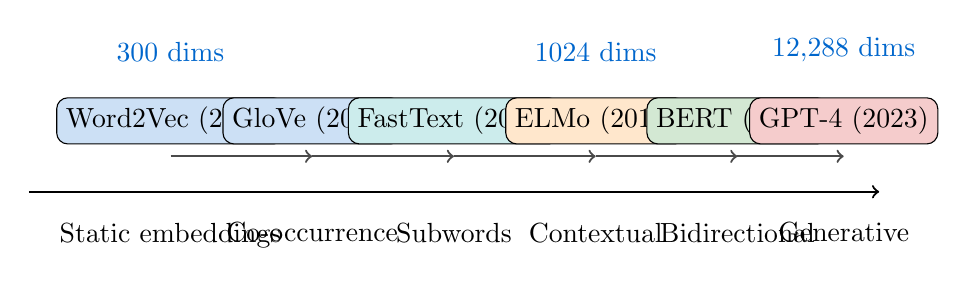
\begin{tikzpicture}[scale=0.9]
% Timeline
\draw[thick, ->] (0,0) -- (12,0) node[anchor=north] {};

% Word2Vec era
\node[draw, fill=ChartBlue!20, rounded corners] at (2,1) {Word2Vec (2013)};
\node[below] at (2,-0.3) {Static embeddings};
\node[above] at (2,1.7) {\data{300 dims}};

% GloVe
\node[draw, fill=ChartBlue!20, rounded corners] at (4,1) {GloVe (2014)};
\node[below] at (4,-0.3) {Co-occurrence};

% FastText
\node[draw, fill=ChartTeal!20, rounded corners] at (6,1) {FastText (2016)};
\node[below] at (6,-0.3) {Subwords};

% ELMo
\node[draw, fill=ChartOrange!20, rounded corners] at (8,1) {ELMo (2018)};
\node[below] at (8,-0.3) {Contextual};
\node[above] at (8,1.7) {\data{1024 dims}};

% BERT
\node[draw, fill=DarkGreen!20, rounded corners] at (10,1) {BERT (2018)};
\node[below] at (10,-0.3) {Bidirectional};

% GPT
\node[draw, fill=DarkRed!20, rounded corners] at (11.5,1) {GPT-4 (2023)};
\node[below] at (11.5,-0.3) {Generative};
\node[above] at (11.5,1.7) {\data{12,288 dims}};

% Arrows showing evolution
\draw[->, thick, DarkGray] (2,0.5) -- (4,0.5);
\draw[->, thick, DarkGray] (4,0.5) -- (6,0.5);
\draw[->, thick, DarkGray] (6,0.5) -- (8,0.5);
\draw[->, thick, DarkGray] (8,0.5) -- (10,0.5);
\draw[->, thick, DarkGray] (10,0.5) -- (11.5,0.5);

\end{tikzpicture}
\end{center}

\vspace{8mm}

\begin{columns}[T]
\column{0.48\textwidth}
\textbf{Word2Vec's Legacy:}
\begin{itemize}
\item Proved embeddings work
\item Inspired contextual models
\item Still used in production
\item Foundation for all modern NLP
\end{itemize}

\column{0.48\textwidth}
\textbf{What Changed:}
\begin{itemize}
\item Static → \success{Contextual}
\item 300 dims → \success{12,000+ dims}
\item Word-level → \success{Subword}
\item Millions → \success{Billions} of parameters
\end{itemize}
\end{columns}
\end{frame}

% Building semantic search
\begin{frame}[fragile]{Build It: Semantic Search Engine}
\begin{columns}[T]
\column{0.58\textwidth}
\begin{lstlisting}[language=Python]
import numpy as np
from gensim.models import Word2Vec

def semantic_search(query, documents, model):
    """Find semantically similar documents"""

    # Vectorize query
    query_vec = document_vector(query, model)

    # Vectorize all documents
    doc_vectors = [
        document_vector(doc, model)
        for doc in documents
    ]

    # Compute similarities
    similarities = [
        cosine_similarity(query_vec, doc_vec)
        for doc_vec in doc_vectors
    ]

    # Return ranked results
    ranked = sorted(
        zip(documents, similarities),
        key=lambda x: x[1],
        reverse=True
    )

    return ranked[:10]  # Top 10 results

def document_vector(text, model):
    """Average word vectors for document"""
    words = text.lower().split()
    vectors = [
        model.wv[word]
        for word in words
        if word in model.wv
    ]
    return np.mean(vectors, axis=0)
\end{lstlisting}

\column{0.40\textwidth}
\textbf{How it works:}
\begin{enumerate}
\item Convert query to vector
\item Convert documents to vectors
\item Find nearest neighbors
\item Return ranked results
\end{enumerate}

\vspace{8mm}
\textbf{Real Examples:}

Query: "animal pets"

\success{Results:}
\begin{itemize}
\item "dog training tips"
\item "cat care guide"
\item "hamster habitats"
\end{itemize}

\vspace{5mm}
\secondary{No keyword matching needed!}
\end{columns}
\end{frame}

% Summary
\summaryslide{Week 2 Summary: Words Have Meaning!}{
\begin{itemize}
\item Words as \highlight{IDs} → Words as \highlight{vectors}
\item Distributional hypothesis: \data{Context defines meaning}
\item Word2Vec: \success{Skip-gram} + \success{Negative sampling}
\item Mathematical semantics: King - Man + Woman = Queen
\item From 50,000 sparse → \data{300 dense} dimensions
\item Powers modern NLP: Search, translation, chatbots
\item Limitations led to BERT/GPT development
\end{itemize}

\vspace{10mm}
\textbf{Key Technical Insights:}
\begin{itemize}
\item Dot product captures similarity
\item Negative sampling avoids softmax bottleneck
\item Embeddings are the foundation of all modern NLP
\end{itemize}

\vspace{10mm}
\textbf{Next Week:} Recurrent Neural Networks\\
\secondary{How do we process sequences using embeddings?}
}

\end{document}